% template d'article LaTeX créé par Max De Wilde (STIC - ULB)
% contact : madewild@ulb.ac.be

\documentclass[a4paper,12pt]{article} % ce document est un article sur une feuille A4, police taille 11

\usepackage[utf8]{inputenc} % encodé en utf-8
\usepackage[T1]{fontenc} % compatible avec les accents

\usepackage[round]{natbib} % gestion des citations
\usepackage[french]{babel} % rédigé en français
\usepackage[hyphens]{url} % formatte les liens en autorisant la césure au niveau des traits d'union
\usepackage[pdftex,urlcolor=black,colorlinks=true,linkcolor=black,citecolor=black]{hyperref} % liens cliquables mais non colorés
\usepackage[top=3cm,bottom=4cm]{geometry} % gère les marges
\usepackage{graphicx} % gestion des images
\usepackage{array} % gestion des tableaux
\usepackage{csquotes} % gestion des guillemets
\usepackage{fourier} % utilise une autre police que celle par défaut (Computer Modern)

% insérez ici d'autres extensions avec la commande \usepackage[options]{nom de l'extension}

\title{\textbf{La reconnaissance d'objets intra-images}} % le titre de l'article
\author{VANBELLE Julien} % vos prénom et nom
\date{} % pas de date

\begin{document} % début du corps du texte
\maketitle % affiche le titre, l'auteur et la date

\begin{figure}[h] % insère une figure ici (h = "here")
  \centering % centre la figure
  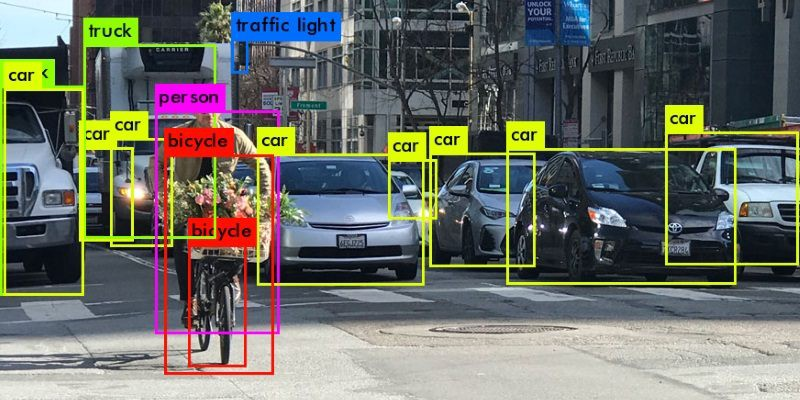
\includegraphics[scale=0.5]{illu1.jpg} % insère une image en taille réelle
  % l'extension n'est pas précisée pour éviter des problèmes de compilation
  % plus d'info ici : http://fr.wikibooks.org/wiki/LaTeX/Inclure_des_images
  \caption{Source: https://www.datagenius.fr/post/reconnaissance-d-image-intelligence-artificielle-ai-compare} % nom de l'image
\end{figure}
\vspace{40}
\section{Plan du document}
\begin{enumerate}
    \item Introduction (p. XX - XX) \newline
    \item Principes de bases (p. XX - XX)\newline
    \item La reconnaissance d'objets dans un flux d'images(p. XX - XX)\newline
    \item Conclusion (p. XX - XX)\newline
\end{enumerate}
               \newpage
\section{Introduction} % section 1
		Parmi les sens présents chez l'être humain, notre vision constitue le sens le plus critique quand il s'agit d'interagir avec notre environnement. De nos jours, la quasi omniprésence du numérique amène des nouveaux défis, notamment dans la gestion numérique de l’environnement réel. Ce défi s’intitule « la vision par ordinateur » et il constituera le sujet de ce travail. \newline

	Nos interactions et notre compréhension du monde qui nous entoure repose, en autre, sur notre vision, un sens que l’on a appris à maitriser depuis notre plus jeune âge mais qui reste relativement complexe pour une machine. En effet, si nous somme capable de reconnaître en un coup d’œil un objet qui nous est familier, comment pourrais faire une machine pour nous égaler ? 
Avant de reconnaître un objet, il faut avant tout le connaître ou plutôt l’apprendre à un ordinateur. Pour cela, il faut s’intéresser à la caractérisation des objets présent dans notre environnement quotidien.  Plusieurs méthodes de caractérisation sont possibles, on pourrait définir un objet par son contour général ou par l’image de l’objet dans sa globalité ou encore via des parties de l’image de cet objet. L’ensemble de ces méthodes seront analysées dans ce travail. \newline

	En ce qui concerne la reconnaissance de ces objets caractérisés, la vision par ordinateur fait appel à différents modèles de ce que l’on caractérise aujourd’hui d’intelligence artificielle. On verra dans ce travail les limites des différentes techniques de machine learning exploitées dans le cadre de la reconnaissance d’objets. On s’intéressera notamment sur la méthode « pixels by pixels », la méthode par modèle de vecteur et les méthodes qui exploitent des réseaux de neurones.\newline

	Actuellement, les techniques de reconnaissance d’objets intra images sont exploitées dans une multitude de domaines différents, par exemple on utilise la vision par ordinateur dans le secteur des soins de santé pour identifier des tumeurs, on l’utilise aussi dans le secteur du transport pour analyser le trafic routier et permettre la genèse d’une génération de voiture autonome. L’agriculture exploite également ces techniques mais aussi le secteur de la défense pour effectuer de la reconnaissance de matériel militaire. Dès lors, on peut déduire vu la variété d’applications de ces techniques que celles-ci vont posséder une place de plus en plus prépondérante dans notre société.\newline
\newpage
\section{Principes de bases}
\textbf{1) L'image numérique }\newline
\begin{figure}[h] % insère une figure ici (h = "here")
  \centering % centre la figure
  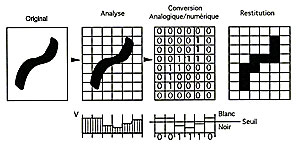
\includegraphics[scale=0.8]{binaire.jpg} % insère une image en taille réelle
  % l'extension n'est pas précisée pour éviter des problèmes de compilation
  % plus d'info ici : http://fr.wikibooks.org/wiki/LaTeX/Inclure_des_images
  \caption{Source: http://www.map.toulouse.archi.fr/works/panoformation
  /imagenum/imagenum.html } % nom de l'image
\end{figure}
\newline
\par
	La majorité des images numériques que nous manipulons aujourd’hui sont caractérisées majoritairement par une représentation matricielle du réel. La représentation numérique d’un réel est donc un ensemble de cases appelé pixels qui restituent les informations de luminosités et de chromaticité d’un point du réel imagé. Nous ne rentrerons pas en détail ici sur le processus de captation d’une image numérique car bien que passionnant il constitue une digression dans le cadre de ce travail. \newline

	Néanmoins, il semble important de préciser une caractéristique propre à l’image numérique. En effet, celle-ci se caractérise par sa résolution que l’on pourrait simplifier par le nombre de points ou pixels que possède une image pour représenter un réel en fonction de l’unité de longueur de cette image. Cette caractéristique peut se révéler importante dans le cadre de la cadre de la détection d’objets car une trop faible résolution pourrait réduire la lisibilité de la forme représentée, mais une trop grande résolution pourrait également augmenter le temps de calcul compte tenu de la quantité de détail et dès lors d’information à traiter. En effet, comme nous pourrons le constater par la suite, certain modèle de reconnaissance d’objet intra image limite les résolutions de traitement afin de conserver une efficacité optimale.  
\newpage
\textbf{2) Reconnaissance générale et spéficique}
\newline
\par
	Dans le domaine de la vision par ordinateur il y a deux types de reconnaissance d'objet dans une image, 
\newpage
\section{État de l'art} % section 2
Le texte de l'état de l'art selon \citet[p. 123]{Boy11}. % une citation avec n° de page
\newpage
\section{Analyse} % section 3
Le texte de l'analyse...\footnote{\url{http://mastic.ulb.ac.be}}

\begin{table}[h] % insère un tableau ici
  \centering % centre le tableau
  \begin{tabular}{|l|c|r|} % insère un tableau avec 3 colonnes centrées à gauche (l), au centre (c) et à droite (r)
    \hline % ligne horizontale
    STIC3 & STIC4 & STIC5 \\ % contenus des cellules séparés par des & et \\ en fin de ligne
    \hline
    STIC3 & STIC4I & STIC5I \\
    STIC3 & STIC4C & STIC5C \\
    \hline
  \end{tabular}
  \caption{Finalités du MaSTIC}
\end{table}
\newpage
\section{Conclusion} % section 4
\newpage
\enquote{Une bonne conclusion est une conclusion finale.} \citep{Hoo12} % citation entre guillemets et auteur entre parenthèses avec \citep

\bibliographystyle{plainnat-fr} % paramètre l'affichage de la bibliographie
\bibliography{biblio} % indique que la bibliographie se trouve dans le fichier biblio.bib

\end{document} % fin du corps du texte